\section{Impact of KID non-linearity}
\label{se:KID_NL}

\subsection{Total power}

In this paragraph we characterize KID non-linearity in total power. To do so, we simulate the observation of a point source by a KID, with a flux that we vary between \todo{1 and 2000\,Jy TBC} (fluxes are unrealistically large on purpose for illustration), to see how linear the measure remains. We assume that our instrument has a 11\,arcsec FWHM Gaussian beam like the polarized 1\,mm channel of \nikad. In the simulation, we use \methodu\ and  \methodd\ to recover the received power. We write the non linear detector response as :

\begin{equation}
m = m + \varepsilon_{det} m^2 +c_{0}.
\label{eq:model_kid_nl}
\end{equation}

\epsDET\ represents the non linearity of the KID. 
For all simulations we compute the non-linearity coefficient \epsDET\ from eq.~(\ref{eq:model_kid_nl}) by doing a linear fit of the input fluxes as a fonction of output fluxes.

Fig.~\ref{fig:planet_profiles} and Fig.~\ref{fig:flux_out_vs_in} show that non-linearity appears with the distortion of the input gaussian profile in the case of \methodu\ whereas \methodd\ remains linear on the same flux scale. \todo{voir pourquoi Cf reste lineaire compare a Rf}

\begin{figure}
  \includegraphics[clip, angle=0, width=\columnwidth]{Figures/planet_profiles_2.eps}
  \caption{Comparison of an incoming flux that we vary between 1 and 2000 Jy TBC (in black), with flux reconstructed by \methodu\ and \methodd. Fluxes are unrealistically large on purpose for illustration. }
  \label{fig:planet_profiles}
\end{figure}


\begin{figure}
  \includegraphics[clip, angle=0, width=\columnwidth]{Figures/flux_out_vs_in.eps}
  \caption{Comparison of an incoming flux that we vary between 1 and 2000 Jy TBC (in black), with flux reconstructed by \methodu\ and \methodd. Fluxes are unrealistically large on purpose for illustration. }
  \label{fig:flux_out_vs_in}
\end{figure}

 Results are shown in Tab.~\ref{tab:eps}. As in the two figures the non-linearity coefficients show \methodu\ method is less linear than \methodd\ on the same flux scale.\\

\begin{table}
\center
\begin{tabular}{|c|c|c|}
	\hline
	    & $\frac{3pts}{beam}$ & $\frac{5pts}{beam}$ \\
	\hline
\methodu\	&  $-4.58 \times 10^{-5}$ & $-2.33 \times 10^{-5}$ \\
	\hline
\methodd\ & $1.09 \times 10^{-7}$   & $8.90 \times 10^{-8}$ \\
	\hline
\end{tabular}
\caption{Non-linearity coefficients \epsDET from an incoming flux that we vary between 1 and 500 Jy.}
\label{tab:eps}
\end{table}


%KIDs are a novel technology successfully used in \nikad . Because of their multiplexing capability and their short time constant, they are one of the best candidates to be implemented on experiments that need larger arrays. In this section we studied KIDs non-linearity and its impact on CMB B mode measures, considering the brightness of a source, the scanning speed of the instrument and the method that we use to follow the shift of the resonant frequency and retrieve the absorbed power.
%Simulations of a KID exposed to a point source with a large variation of fluxes have shown that as expected, the brighter is the source, the more non-linearities appear due to a poor reconstruction of the resonant frequency. Although both reconstruction methods give good results, \methodd\ remains more linear at high fluxes than \methodu . Plus, KID non-linearity should not impact measures of CMB B modes, in fact the non-linearity coefficients that we found are in the range of $[10^{-5} - 10^{-8}]$, so it meets the requirement addressed in Sec.\ref{sec:cmb}.
%In futur CMB polarization experiments, the use of a half wave plate more and more common. It presents a lot of advantages, but can also be source of various systematic effects. In the next section we will address the non-linearity that can arise from rotating a half wave plate in an instrument.




\subsection{Polarization and Half Wave Plate}
\subsubsection{Half Wave Plate}
\subsubsection{Simulations}





